\documentclass{report}

\usepackage{graphicx}
\usepackage{listings}
\usepackage{color}
\definecolor{codeColor}{rgb}{0.4, 0.6, 0.8}
\lstset{keywordstyle=\color{codeColor},language=Octave,stepnumber=1,basicstyle=\footnotesize}

\usepackage{enumitem}

\newenvironment{steps}[1]{\begin{enumerate}[label=#1 \arabic*]}{\end{enumerate}}

\makeatletter
\def\step{
   \@ifnextchar[ \@step{\@noitemargtrue\@step[\@itemlabel]}}
\def\@step[#1]{\item[#1]\mbox{}\\\hspace*{\dimexpr-\labelwidth-\labelsep}}
\makeatother

\begin{document}

\title{ Solucion de Ecuaciones No Lineales}
\author{Rub�n Cuadra A01019102}

\maketitle
\begin{abstract}
	Manual de usuario:  'ortogonaliza.m', el objetivo de este documento es documentar la implementacion de Gram-Schmidt como metodo numericos
\end{abstract}

\section{Introduccion}
	El codigo consiste en un archivo llamado de la misma manera que la funcion el cual recibe 2 argumentos y nos regresa 2 respuestas
\lstinputlisting[ firstline=1, lastline=1]{ortogonaliza.m}

	\textbf{V}  Es un arreglo con vectores que seran ortogonalizados
		
	\textbf{eps} es nuestro criterio para decidir si se agrega como vector ortogonalizado al retorno, este se compara con la magnitud del vector obtenido (Explicacion mas adelante)

\section{Comprension del algoritmo}
	
\subsection{Gram-Schmidt}
Busca generar un conjunto de vectores que genere el mismo subespacio vectorial que los vectores iniciales

El algoritmo usado es: 
\begin {equation}
\mathbf{u}_k = \mathbf{v}_k-\sum_{j=1}^{k-1}{\langle \mathbf{u}_j, \mathbf{v}_k\rangle\over\langle\mathbf{u}_j,\mathbf{u}_j\rangle}\mathbf{u}_j 
\end {equation}

\begin{steps}{Paso}
\step Agregar el Primer vector al retorno $\mathbf{VO}_1 = \mathbf{V}_1,$
\step Generamos un ciclo desde 2 hasta e total de vectores en \textbf{V} (Ya que la posicion 1 ya fue asignada en el paso anterior)
\step Inicializamos una variable $temp = 0$
\step Generamos un ciclo con el total de columnas en $\mathbf{VO} $ de manera que: $temp =\sum_{j=1}^{Col(VO)}{\langle \mathbf{u}_j, \mathbf{v}_k\rangle\over\langle\mathbf{u}_j,\mathbf{u}_j\rangle}\mathbf{u}_j $
\step Obtenemos el vector ortogonal usando ${VO}_i - temp$
\step Comparamos ${\mathbf{u}_k \over \sqrt{\langle\mathbf{u}_k,\mathbf{u}_k\rangle}} > eps$ lo que es equivalente a la magnitud del vector ortonormal
\step Si se cumple: Agregamos el vector orotonomal  a ${VO}_{ultima posicion+1}$
\end{steps}
Al final se regresa ${VO}$ y ${R}$ , donde $R= columnas(VO)$

\begin{figure}
    \centering
    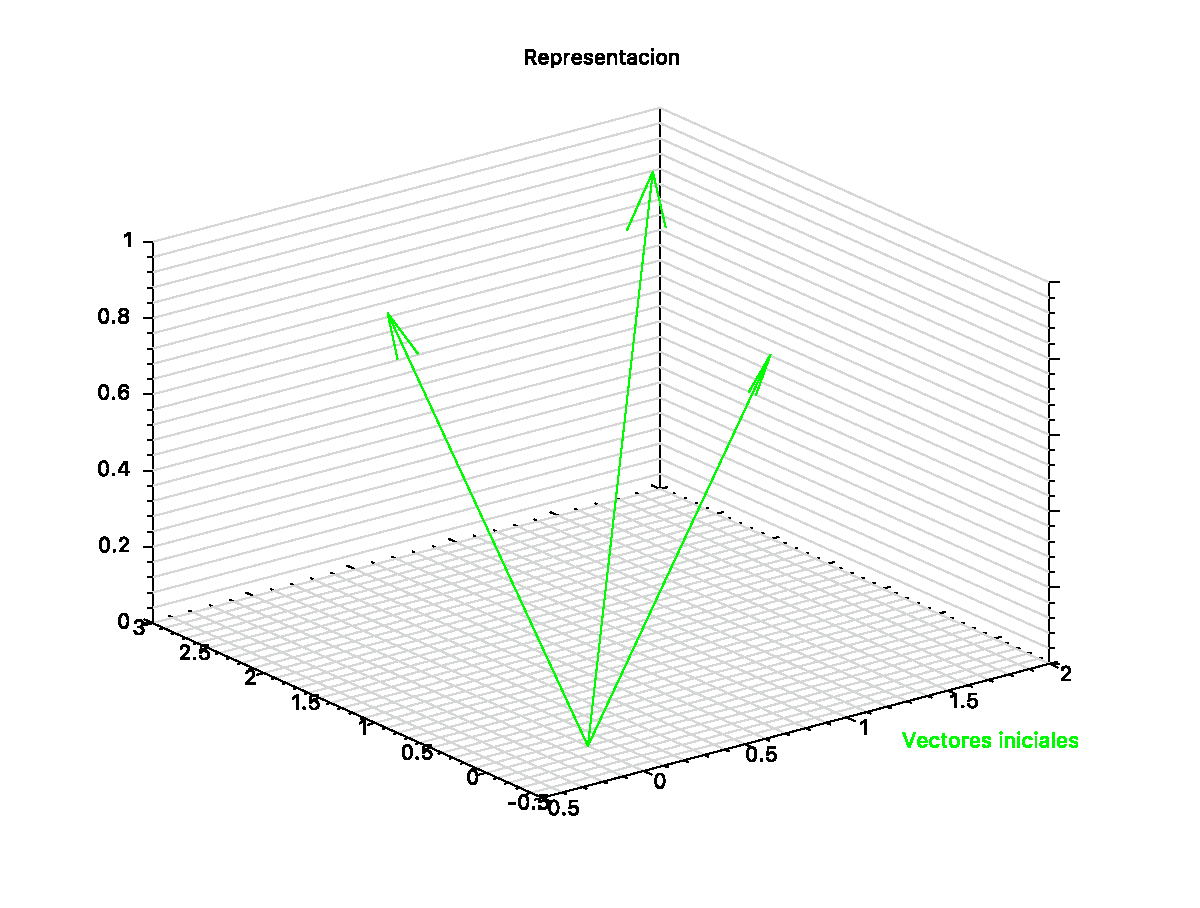
\includegraphics[width=5.5in]{initi}
     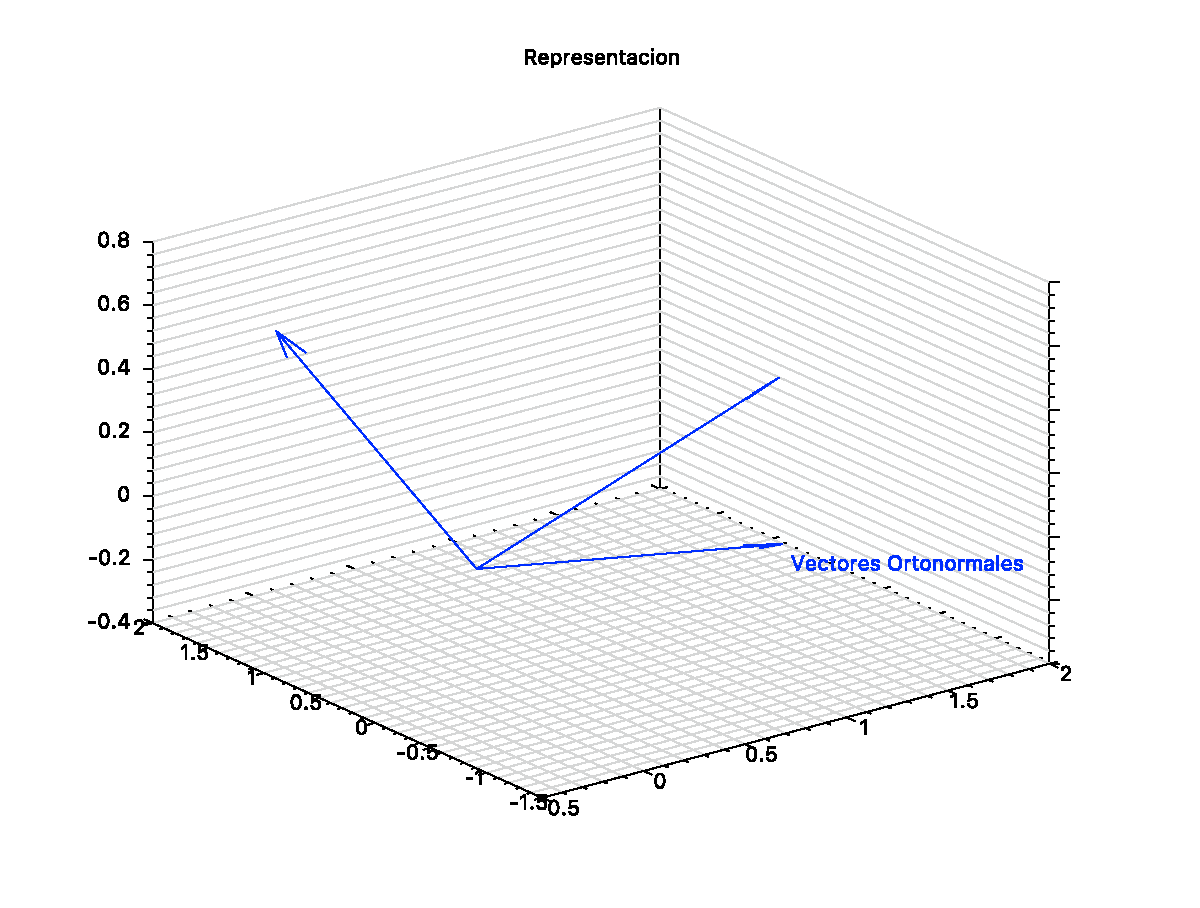
\includegraphics[width=5.5in]{ort}
    \label{examplefigure}
\end{figure}

\section{Ejemplo}
Mandamos a llamar la funcion desde un archivo main.m.
Usando el argumento: 
\lstinputlisting[language=Octave,firstline=1,lastline=1]{main.m}
Llamamos la funcion:
\lstinputlisting[language=Octave,firstline=2,lastline=2]{main.m}
El resultado VO  seria:
\lstinputlisting[language=Octave,firstline=4,lastline=8]{main.m}
y nos devolveria por Rango
\lstinputlisting[language=Octave,firstline=9,lastline=9]{main.m}

Donde VO serian los vectores Ortogonalizados partiendo desde V

\section{Conclusion}
Es un modulo portable que en realidad solo requiere 1 argumento, el eps no es necesario(Pero se puede definir).
\footnotetext{Los acentos no se pudieron agregar por cuestion de la codificacion}

\end{document}
